\chapter{Technical Specification of RESTful Semantic Web services }\label{capituloTS}

\section{Introduction}

In the previous chapter of this document (\ref{capituloFD}) we have introduced a formal theoretical model allowing the description of
semantic restful web services. In this chapter we wil transform this theoretical model in a technical specification
allowing the practical implementation of such a formal model.\\
In this effort great care has been taken into using actual web standards for semantic technologies as well as for the
description of web services. The use of open standards in the specification of a RESTful semantic web services layer
allows easy reusing of existent technologies and software libraries already deployed in present day HTTP agents like web
browsers, ensuring interoperability.\\
The final output of this chapter will be technical description specifying  how to use different existing web standards to
leverage semantic RESTful web services.  In this specification  the following parts of the formal model
must be present:
\begin{itemize}
\item It must specify how to expose the triples containing the meta data of the resource exposed as a RESTful
  semantic web service.
\item It must specify the necessary meta data for a client being able to access the resource through the HTTP uniform
  interface.
\item It must provide a mechanism to transform the resource triplets representation into a concrete syntax in order for clients and
  services to exchange triples through the HTTP uniform interface.
\end{itemize}

One of the main advantages of the REST architectural point of view in the description of web services is its
simplicity. As we have mentioned, this focus on simplicity has been perceived as a reaction to the complexity in the
specification of WS-* style web services. REST principles avoid complexity restricting the expresiveness in the
description of web services to the design principles of the HTTP protocol. Unfortunately, the HTTP protocol  does not include any
standard way to add semantics to the data exchanged through the protocol. In our specification we have tried to add the
minimum necessary overhead on top of REST so these metadata can be automatically exchanged by web agents while staying true to the
simplicity and principles of the HTTP protocol. When dealing with semantic metadata, the main point of interest is the automatic processing of these semantic metadata. We believe  the necessity of automatic processing of the semantic information justifies the use of description languages in a RESTful way, for instance, as metaservices describing the semantics of other services.

\section{State of the Art}
In the world of WS-* web services there has been a great deal of effort in creating effective ways of describing web
services as well as the mechanisms of interaction between services and clients. Standards such as the Web Services
Description Language (WSDL) \cite{w3cwsdl}
offer languages for writing service descriptions that can be automatically processed by client software in order to
generate the necessary code to consume the service.\\
The first version of the WSDL 1.1 specification bindings to the HTTP protocol were inadequate, preventing thus the
description of RESTful web services using this standard. The situation has change with the version 2.0 of the standard
\cite{w3cwsdl2} there have been and improvement of the HTTP bindings allowing the description of WS-* web services with
REST semantics.\\
Outside the standardization efforts of the W3C there have been other proposals fo HTTP based web services description
languages like WADL \cite{wadl}. The main focus of the WADL proposal is in the automatic generation of client code for
accesing the the services resources,  but it has been received with mild
enthusiasm from the RESTful web services developer community and no great adoption of the technology has followed. \\
Main criticism against proposals as the Web Application Description Language (WADL) \cite{greg2007} has come from the observation of the
fact that the complexity in description languages contrast with the alleged simplicity of RESTful web services,
concernings about the RESTful nature of these mechanisms and a perceived lack of sustantial gains in the adoption of the
code generation technologies these languages could enable.\\

In parallel with the advances in the standardization of description languages for web services and RESTful web services,
the W3C semantic web initiative has been fruitful in the generation of standards for the description of semantic
metadata on the web.\\

The foundation of the semantic technologies from the W3C is the Resource Description Framework (RDF) specification \cite{Hayes:04:RS}. RDF describes a
data model allowing anyone ot insert into a HTTP accesible resources assertions about any other web resource designated
after its URI. The resources linked through this assertions conforms a graph of resources that RDF serializes as a set
of triples with subject, predicate and object. This graph can also be serialized, for instance,  as an XML document \cite{rdfxml} and
exposed as a web resource with its own URI. RDF serves as a good foundation for adding simple semantic
descriptions. More complex and expressive ways of adding metadata  have been proposed later as new specifications built
on top of the RDF data model. These specifications were aimed at the specification of ontologies for web resources
allowing inference. The
first of these standard is RDF Schema \cite{Brickley:04:RVD} which provides a set of ontological primitives that can be
annotated to web resources using the RDF data model. The limited expresiveness of RDF Schema lead to the proposal of the
Ontolgy Web Language (OWL) \cite{Dean:04:OWO} in its three version OWL Lite, Full and DL. These last specification has
its roots in the field of description logics and offers a vocabulary for the building of ontologies around web
resources, with well defined semantics.\\

The standardization of these semantic technologies has made possible a whole new kind of software applications in recent
years and has obtained a considerable success. Its adoption nevertheless has not reached its full extent. In a way that
resembles the situtaion happened with WS-* specifications, many users have perceived specifications as OWL as too complex for
use cases not involving inference. Independent proposals for adding semantic metadata into web resources have appeared,
the one meeting the most success being the Microformats initiative. Microformats are small patterns of HTML describing
common entties in the web. They try to provide some of the benefits that can be obtained from the use of the standard
semantic languages avoiding its complexity. The microformats ad-hoc nature nevertheless presents several important drawbacks,
like the lack of a formal model for the description, or the unability to use name spaces in the descriptions.\\

In spite of its limitations, the microformats proposal has met a certain degree of success between web application
developers, helping to bridge the gap between the standar semantic technologies and the web application developers
community. This success has motivated in the last months that the W3C standarized Annotated RDF (RDFa)  \cite{rdfa} as
a standard way of inserting RDF graphs into HTML pages. Support for the indexing of microformats and RDFa documents has
been announced by different search engines companies as Google.\\

Web services and semantic web standards have had a confluence in recent work in the technical specification of a
semantic web services specification language. Between the different proposals submitted for their standarization to the
W3C we can found the  Web Service Modeling Ontology (WSMO) \cite{wsmo}, Semantic Markup for Web Services (OWL-S) \cite{owls}.\\ 
WSMO is the most evolved specifcation, related to sub projects as the Web Service Modeling Langauge (WSML) \cite{wsml}
and the Web Service Modelling Execution Environment \cite{wsmx}. This set of specifications provides a reference model
(WSMO), a syntax (WSML) and a standard implementation (WSMX) of the necessary technologies for specifying and building
semantic web services. In the other hand, OWL-S provides an alternative model for the description of semantic web
services but relies in the standard mechanisms of OWL for the specification of the elements of the service instead of
creating a new one as WSMO does with WSML. \\

Both specifications provide rich models for the description of semantic web services. These conceptual models needs to
be transformed into an exchange syntax and transmitted through a communication channel using a certain communication
protocol, so the information contained in these model can be exchanged between agents. The problem of solving this
abstraction gap is known as grounding into service oriented architectures jargon. The main aspects of web services
grounding can be splitted into data grounding and behavioural grounding \cite{ISBN:3540345191}. Data grounding
transforms the information retrieved from the service into a serialization format. WSMO and OWL-S uses XML as the
encoding  of these messages. Behavioural grounding provides the information necessary for a client to know how to invoke
a service and what kind of messages it should send and receive. WSMO and OWL-S provide their own solution for this
problem involving an interaction model, an abstract state machine in the cas of WSMO, and some XML encoded information
about the kind of messages that can be sent in and out of the service. OWL-S tries to reuse the existent WS-*
techologies providing a mapping from its conceptual model to these technologies. The same approach has been followed by
other W3C submission proposals as the Semantic Web Services Description Language (WSDL-S) \cite{wsdls} consisting in
a lightweight layer of semantic annotations for the components of WSDL.

Up to this point the main poposals for semantic web services have been reviewed. We have noted how they try to join the
world of WS-* web services and W3C standards for the semantic web. We have also taken into account how these standards
have sometimes met criticism for their complexity and have been found unsuitable for certain kind of applications,
spawning lightweight approachs to the same problems as is the case of REST for web services and the microformats
initiative in the case of the W3C standards. We have also seen how this simpler proposals have been integrated in
different ways into the standards as is the case of WSDL 2.0 for WS-* web services and RDFa for semantic metadata.\\

In the world of semantic web services, similar provisions about the complexity of the technologies have started to be
taken. Most notably WSMO has produced reduced versions of the WSMO standard aiming to reduce its complexity: WSMO Lite
\cite{wsmolite} and MicroWSMO \cite{microwsmo}.\\

Both working drafts sketch a reduced WSMO model suitable for simpler web services. MicroWSMO is of an special interest
due to the reason that it tries to adapt the WSMO model to the construction of RESTful semantic web services. As a
complement of the MicroWSMO minimal model another specification knowns as hRESTS has been drafted proposing a vocabulary
expressed as a microformat or a RDFa encoded set of WSML statements for the description of MicroWSMO semantic web
services. \\

From this point of view MicroWSMO/hRESTS is similar to other mechanisms for extracting metadat from a HTML web resource
attaching a transformation mechanism, as the W3C recommendation Gleaning Resource Descriptions from Dialects of
Languages (GRDDL) \cite{Connolly:07:GRD}\\

In this document we will use the MicroWSMO/hRESTS standard proposal, as the basis of our technical description of RESTful semantic web services.

\section{hRESTS description mechanism}

The main aim of hRESTS is to offer a simple way of describing RESTful web services semantics. The ease of use of hRESTS originates in the minimality of the service model described, which has only four basic elements:

\begin{enumerate}
  \item service: the RESTful web services being described
  \item operation: the action that a client can perform in the server
  \item input message: the information sent to the service when performing an operation
  \item output message: the information received from the service after an operation is performed
\end{enumerate}

Each operation is described using the HTTP uniform interface stating the HTTP method and an address consisting of an URL template. This information is asserted as a RDF graph, reusing the vocabulary of the WSMO-Lite semantic web services framework.

\subsection{semantic information in hRESTS}
Semantic metadata are added to the service description in hREST through the description of input and output messages. These elements of the service model allow the assertion of the model of the resource being retrieved or modified.\\
Within the model information there are also links to the description of the necessary transformations to translate the information of the data model into the syntax of the message exchanged between client and server. These transformations are known as lowering (from the model to the exchange syntax) and lifting (from the exchange syntax to the model).

\begin{figure}[htb!]
\centering%
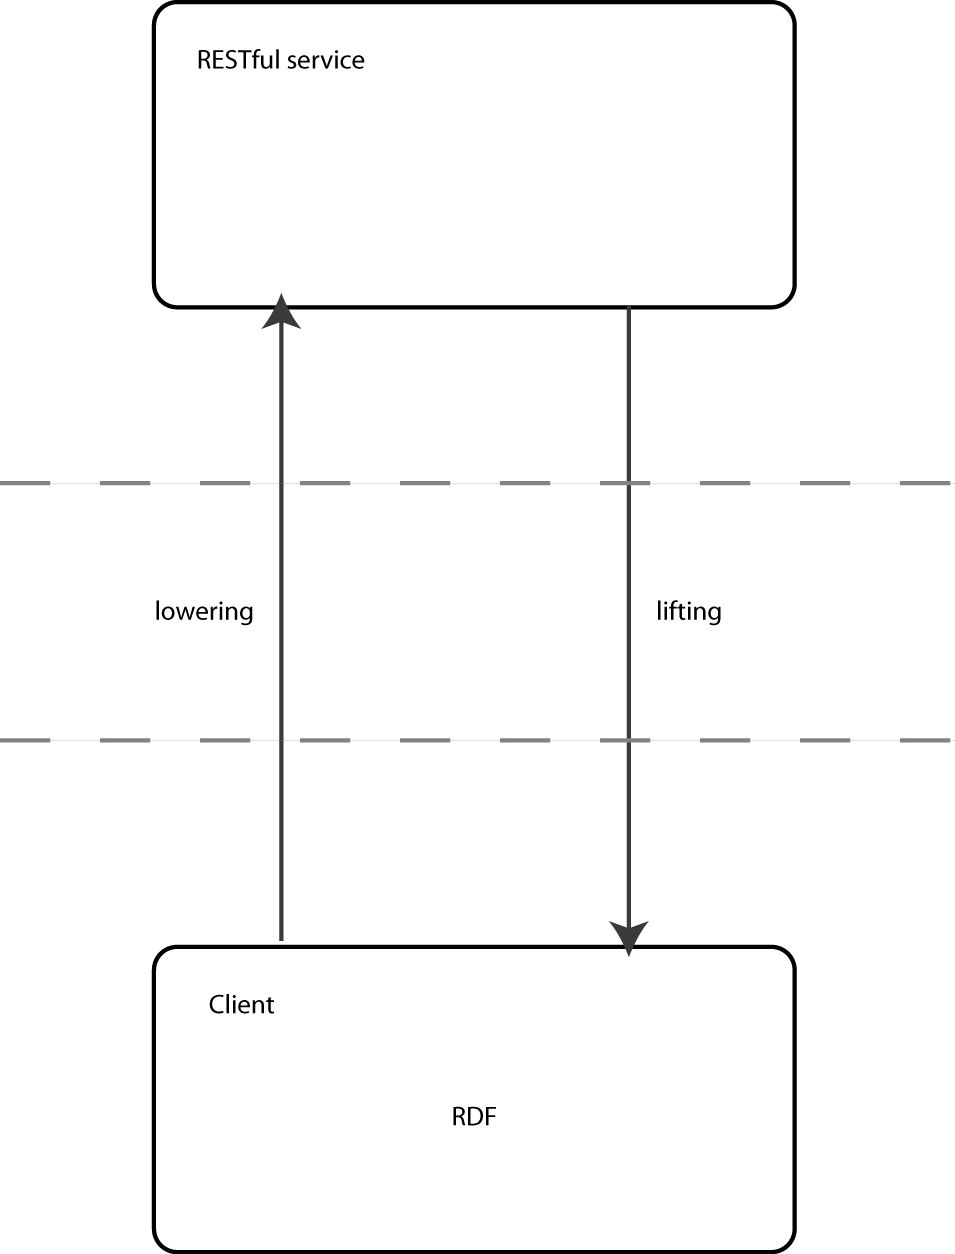
\includegraphics{lifting_lowering.png}
\end{figure}

hRESTS does not specifies a mandatory mechanism for lifting and lowering resources, but offers a mechanism to link the description of the transformations into the service description.

\subsection{encoding of hRESTS descriptions}
A valid hRESTS service description is a RDF graph and thus can be encoded in different formats. All these formats are equivalent for a hRESTS service description, but the proposed encodings for hREST are based in the encoding of the service RDF graph into plain HTML documents. The use of annotated HTML descriptions is the preferred way of describing actual RESTful web services. hRESTS proposes the use of a microformat for inserting the RDF information in these documents. Another proposed mechanism is the use of RDFa \cite{rdfa}, a new W3C standard that makes easy the insertion of RDF graphs inside of XHTML documents.\\
Both encodings have advantages and disadvantages. The use of microformats is a well stablished way of addig semantic information in the development of web applications, and it has big support from the RESTful services community, although it lacks normative recognition and does not have support for namespaces. RDFa on the other hand, is a standard proposal backed by the W3C and also has support for namespaces, but lacks adoption and browse support.\\
Other encodings for hRESTS RDF graphs as YAML and JSON, not covered in the original hRESTS work are explored in this chapter.

\section{hRESTS Grounding}
In this paper a possible grounding mechanism for semantic RESTful web services will be described. \emph{Grounding} is the part in any web services architecture, acting as link between semantic and syntactic descriptions of web services \cite{ISBN:3540345191}, and in the case of \emph{data grounding} how the syntax of a message containing  a representation for that service can be transformed into its semantic counterpart or the other way round.\\
Both transformations, from syntactic representation to semantic representation and from semantic representation to syntactic representation, are commonly called \emph{lifting} and \emph{lowering} as in the W3C recommendation: 'Semantic Annotations for WSDL and XML'' (SAWSDL)  \cite{Lausen:07:SAW}. Lifting and lowering operations present a major difficulty in the specification of semantic web services architectural models. Frameworks like WSMO \cite{wsmo} or OWL-S  \cite{owls} have addressed this issue in different ways. Most of these solutions involve a mixture of XML transformation technologies like XSLT, with web services specific recommendations like WSDL \cite{w3cwsdl} or the aforementioned SAWSDL. Other technologies like XPath \cite{xpath} and XQuery \cite{xquery} are also used. There are  W3C standards like GRDDL (Gleaning Resources Descriptions from Dialects of Languages) \cite{Connolly:07:GRD} specifically created to ease the burden of the tranformation between XML syntactic description of a service and its RDF representation in the semantic model. Other non standardised proposals such as XSPARQL \cite{xsparql} has been created seeking to offer more flexible mechanisms for the translation between XML and RDF.\\
Most of these standards are complex specifications created in the tradition of existing WS-* description mechanisms. They can be used as useful grounding mechanisms for the description of semantic RESTful web services but the particular characteristics of this kind of web services would make desirable a lighter and simpler mechanism for RESTful web services grounding. This paper aims to describe such a mechanism, built over the foundation of existing web grounding technologies.\\

\section{Existent semantic web services grounding mechanisms}
In this section the main existing alternatives for the grounding of semantic web services will be briefly reviewed

\subsection{SAWSDL, WSDL2.0 and HTTP Binding}
WSDL2.0 describes a possible binding for the WSDL components of operation, input and output messages to HTTP concepts \cite{w3cwsdl2}. The following devices are used:
\begin{itemize}
  \item HTTP request IRI location is used as a template for input message in a WSDL operation
  \item HTTP headers are used as a possible binding for the input and output messages of a WSDL operation
  \item Selection of an encoding mechanism for the input and output messages between application/x-www-form-urlencoded, multipart/form-data and application/xml
\end{itemize}
These WSDL concepts and their HTTP bindings can be decorated with SAWSDL annotations. These annotations identify the semantic model involved in the WSDL operation and the transformation mechanisms between the XML representation of the service and the semantic model. SAWDSL does not enforce a certain semantic modelling language. The only requirement made is that concepts from the semantic model should be identified by an IRI. In the same way, any transformation mechanism can be associated to the input and output components of WSDL throught the lifting and lowering constructs of SAWDL. Possible transformation mechanisms are XSLT, XQuery, SPARQL \cite{sparql} or XSPARQL \cite{xsparql}.
In figures 1 to 3, conceptual relations between the different standards used in the grounding mechanism, from HTTP to SAWSDL, are shown.

\begin{figure}[htb!]
\centering%
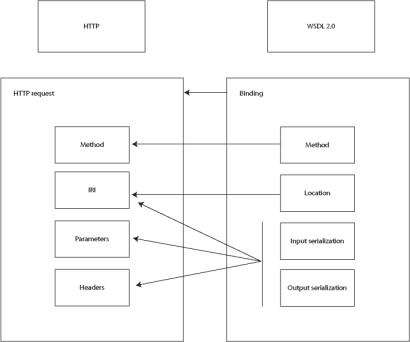
\includegraphics{wasdl1.png}
\caption{WSDL to HTTP mapping}
\end{figure}

\begin{figure}[htb!]
\centering%
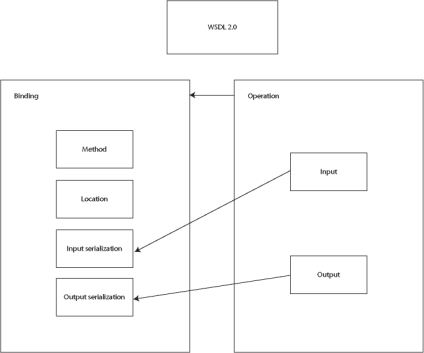
\includegraphics{wasdl2.png}
\caption{WSDL to WSDL HTTP binding}
\end{figure}

\begin{figure}[htb!]
\centering%
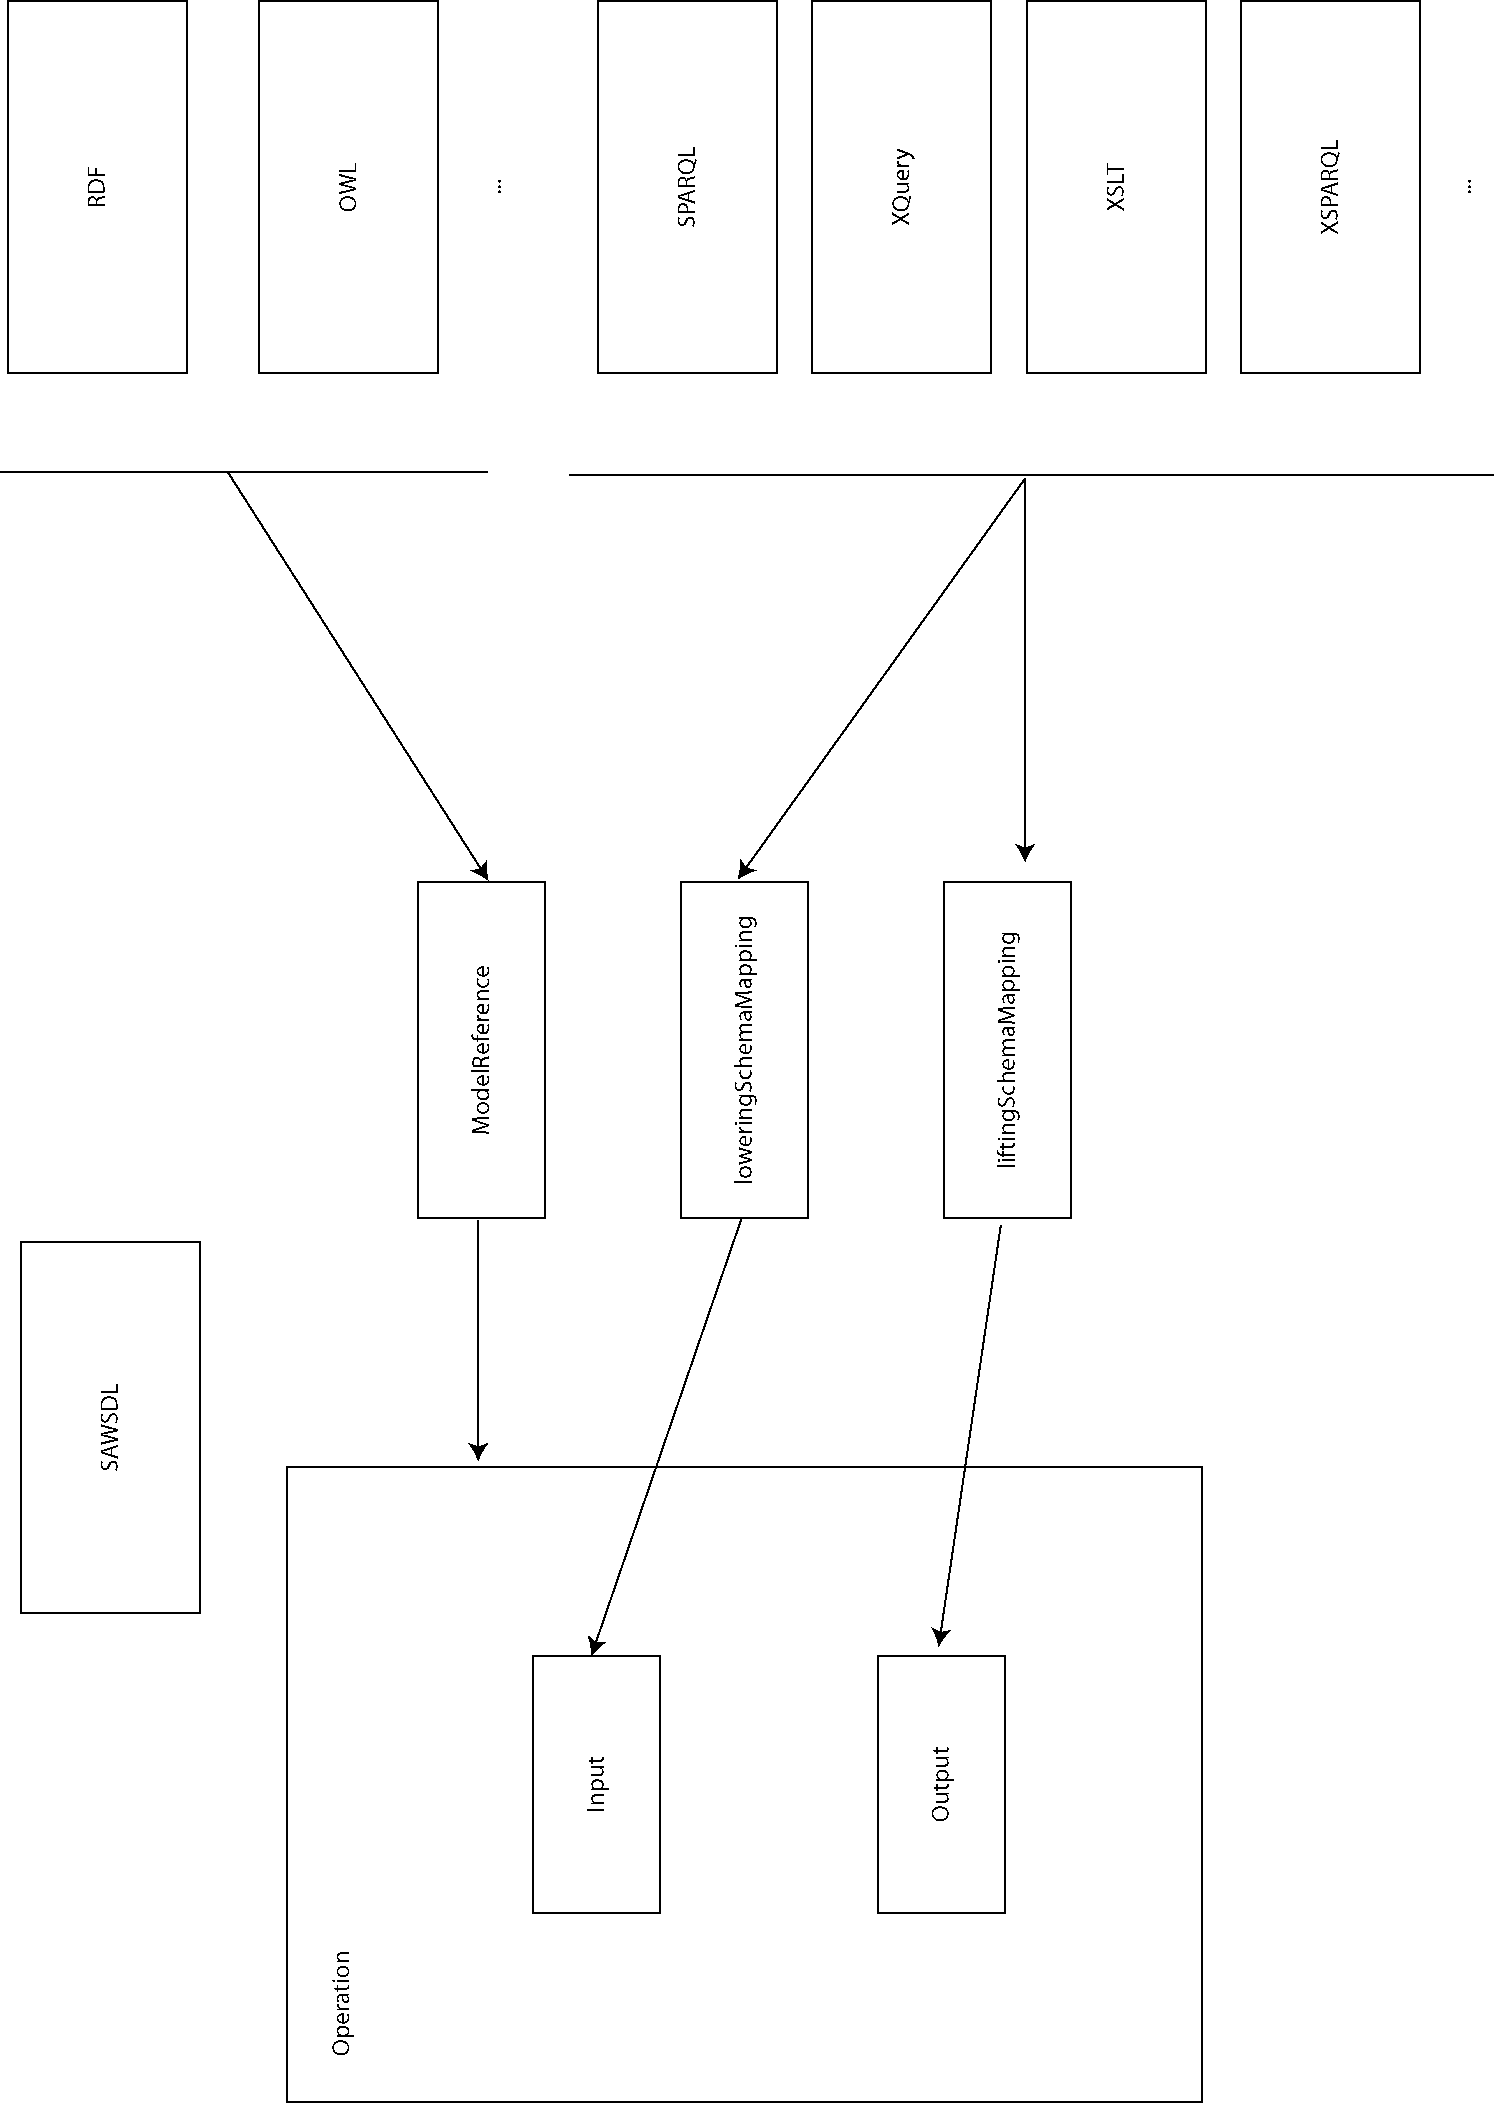
\includegraphics{wasdl3.png}
\caption{SAWSDL annotations}
\end{figure}

\subsection{WSMO Lite and OWL-S}
WSMO Lite \cite{wsmolite} has been conceived as a semantic layer over WSDL but no grounding mechanism is included into WSMO Lite. The ontology for describing semantic web services in WSMO Lite can be transformed into WSDL by means of an annotations mechanism. SAWSDL is proposed as the chosen mechanism but any other semantic annotations language could be used.\\
In the case of OWL-S, this semantic ontology for web services is situated in a similar conceptual relation to WSDL as WSMO Lite. Nevertheless, in this case, the annotation mechanism is included in the ontology vocabulary. This is accomplished by the insertion of OWL-S WsdlGrounding class instances. These elements define XSLT transformations for the input and output messages of WSDL.

\subsection{Transformation languages}
As we have seen, every grounding specification ultimately relies on a transformation mechanism describing how an original model must be transformed into a destination model. The original and destination models can be the semantic model of the object or the returned XML description of the data retrieved. There exists different standard models to describe such transformations, like XSLT or XQuery. All these technologies are complementary and can be used together to obtain more expressive tranformation models.

\begin{itemize}
\item \bf{XSLT}
\end{itemize}

XSLT \cite{xslt} describes a set of constructs arranged in a stylesheet to tranform in a functional fashion XML documents into different XML documents. XSLT can be used in a lowering operation to transform a XML document containing a serialization of a RDF graph into a XML document with the syntax accepted by the service. For lifting operations the XML document returned from the service could be transformed by a XSLT stylesheet into XML/RDF.\\
The support for XSLT is quite mature and every major web browser has support for XSLT tranformations.

\begin{itemize}
\item \bf{XPath}
\end{itemize}

XPath is a standard language which allows the user to specify selections of certain parts in a XML document. XPath grants a set of operations and basic functions that can be applied to path expressions to match parts of the XML document. XPath alone cannot be used as a lifting and lowering mechanism, but it is a basic building block for different transformation languages like XSLT. The current support for XPath in browsers and other tools is fairly good and mature implementations of the standar are available.

\begin{itemize}
\item \bf{XQuery}
\end{itemize}

XQuery is a full programming language, embeddable in XML documents, that allows the retrieval of parts of a document, its transformation, and the creation of new XML documents based on the processed data. XQuery overlaps to a certain degree with XSLT, but while XSLT is a stylesheet language XQuery was conceived as a more general language for retrieving and processing information from other sources than XML documents, like SQL databases. There are numerous implementations of XQuery, but the complexity of the language currently prevents its implementation in many applications like commercial browsers. XQuery can be used alone to specify any kind of transformation in the lifting and lowering operations of a web service.

\begin{itemize}
\item \bf{SPARQL}
\end{itemize}

SPARQL is the standard way of retrieving triplets from RDF graphs. It offers a query language similar to SQL where variables are declared along with query modifiers. As a result, a set of bindings for those variables is obtained from the RDF repository or graph when the query is processed. SPARQL also offers constructs to build new graphs from SPARQL queries. SPARQL can be used in combination with a tranformation language to offer a complete lifting and lowering mechanism.

\begin{itemize}
\item \bf{XSPARQL}
\end{itemize}

XSPARQL is a recent proposal for a transofmation mechanism specifically conceived to ease the tranformation between RDF and different XML formats. It has been conceived  with lowering and lifting operations necessities in mind. XSPARQL can be described as a mixture of SPARQL query capabilities with the XQuery syntax. The flexibility of SPARQL allows a easier retrieval of information from RDF graphs that can be later processed with XQuery constructs. These features made up for a powerful lifting and lowering mechanism. Nevertheless, XSPARQL hast not been yet submitted as a recommendation proposal and its support by tools is almost non existent.

\begin{itemize}
\item \bf{GRDDL}
\end{itemize}

GRDDL is not a transformation language per se, but a standardized way of linking the transofmations required for retrieving RDF metadata from a XML document. GRDDL can be used as a flexible lifting mechanism since it can be used in combination with any other transformation language.

\section{Applicability to semantic RESTful web services}

In the previous section we have reviewed the main existent transformation mechanisms for lowering and lifting operations. Most of these mechanisms have been conceived as generic transformation models and thus are directly reused by the grounding mechanisms of frameworks like WSMO Lite and OWL-S. These specifictions seek to enable the semantic description of any kind of web service but their application to the description of RESTful web services raise some issues that need to be solved.\\

\begin{itemize}
  \item lowering operations in RESTful web services does not generally involve generating XML documents as output but binding certain values from a RDF graph into parts of the URL or header of the HTTP request. This greatly renders XML transformation languages as XSLT unsuitable for this task.
 \item the semantic model in RESTful web services, involved in lifting and lowering operations, is not generally available for a REST client as XML encoded representation of the graph, but by some kind of abstract model stored in a RDF repository. It is easier for a client to access directly this RDF repository with a query language like SPARQL, that building an intermediary XML encoded representation of the graph that would be later transformed by a XSLT or XQuery transformation. It is possible to directly query the repository using XQuery but is not an easy task without the help of specific XQuery libraries \cite{xquery}. XSPARQL seems to simplify this particular task but its specification status is still far away from being standardised.
\item RESTful web services often return as a result other representations different from XML. It is general practise the use of lightweight data representations like JSON \cite{json}, specially for those RESTful services intended to be consumed from javascript clients. This outputs cannot be processed, in the context of a lifting operation, by transformation languages of XML documents.
\item Lightweight RESTful web services clients, for instance, javascript clients executing in a browser, have limited computational resources preventing them from executing runtimes for complex transformation mechanisms like XQuery.
\item Semantic web services frameworks like WSMO Lite and OWL-S choose WSDL as the final step of their grounding mechanisms. Despite the WSDL 2.0 capacity of binding its service model to the HTTP protocol, the use of WSDL with a SOAP binding is perceived as contrary to REST principles and cumbersome by many developers.
\end{itemize}

All these limitations does not prevent the building of semantic RESTful web services with the previous technologies, but this issues must be addressed in order to achieve a fully functional service. In the following sections we will take a look at different ways of easing the burden of specifying the grounding mechanism for RESTful web services.

\section{Grounding mechanism proposal for RESTful semantic web services}

In the following sections a grounding mechanism for RESTful semantic web services will be described. This grounding mechanism tries to overcome the limitations of the currently available mechanisms. 

\subsection{Desired features of a grounding mechanism for RESTful semantic web services}

In order to specify a good grounding mechanism for RESTful web services, there exists a set of features that must be met by such an specification. 

\begin{itemize}
  \item Grounding mechanisms must be able to deal with different representations of data in lifting and lowering operations. They must have support for XML representations of messages but also for JSON, and they must provide a way to exchange binary messages between client and server.
  \item It must offer a binding mechanism to the HTTP components. HTTP verbs, headers and status code must retain its original semantics in the binding mechanism.
  \item The semantic model where information will be stored and later retrieved is assumed to be some kind of triplet repository capable of storing a RDF graph. Thus the preferred method for retrieving data from the semantic model will be SPARQL.
   \item It should be possible to embed grounding information into a XHTML document, whether by the use of RDFa or by the use of microformats.
   \item The grounding mechanism should be extensible enough to allow the attachment of different transformation technologies if necessary to express services not following RESTful principles.
   \item Standard W3C recommendations should be used where possible.
   \item The grounding mechanism should be suitable to be used by lightweight clients, like web applications being executed inside a web browser with limited computational power.
\end{itemize}


\subsection{hRESTS semantic web framework grounding mechanism}

We have already explored in previous papers the mixture of hRESTS and Micro WSMO \cite{hrests} to obtain a framework for describing semantic RESTful web services. hRESTS is built with standard tags extracted from other standard semantic web services frameworks like WSMO Lite and standards like SAWSDL. In the following listing relevant tags for marking down semantic information with hRESTS are shown.
\vspace{5 mm}
\begin{lstlisting}
@prefix hr: <http://www.wsmo.org/ns/hrests#>. 
@prefix rdf: <http://www.w3.org/1999/02/22-rdf-syntax-ns#>. 
@prefix rdfs: <http://www.w3.org/2000/01/rdf-schema#>. 
@prefix wsl: <http://www.wsmo.org/ns/wsmo-lite#>. 
@prefix xsd: <http://www.w3.org/2001/XMLSchema#>. 
@prefix sawsdl: <http://www.w3.org/ns/sawsdl#>.

wsl:Service a rdfs:Class. 
wsl:hasOperation a rdf:Property; 
  rdfs:domain wsl:Service; 
  rdfs:range wsl:Operation. 
wsl:Operation a rdfs:Class. 
wsl:hasInputMessage a rdf:Property; 
  rdfs:domain wsl:Operation; 
  rdfs:range wsl:Message. 
wsl:hasOutputMessage a rdf:Property; 
  rdfs:domain wsl:Operation; 
  rdfs:range wsl:Message. 
wsl:Message a rdfs:Class. 
 
hr:hasAddress a rdf:Property; 
  rdfs:domain wsl:Operation; 
  rdfs:range hr:URITemplate. 
hr:hasMethod a rdf:Property; 
  rdfs:domain wsl:Operation; 
  rdfs:range xsd:string. 
 
hr:URITemplate a rdfs:Datatype. 

sawsdl:modelReference a rdf:Property
  rdfs:domain wsl:Message
sawsdl:loweringSchemaMapping a rdf:Property
  rdfs:domain wsl:Message
sawsdl:liftingSchemaMapping a rdf:Property
  rdfs:domain wsl:Message
\end{lstlisting} \vspace{5 mm}

From this ontology, the properties involved in the grounding mechanisms are the following ones:

\begin{itemize}
  \item \emph{hr:hasAddress} Defines an URI template where parts of this template should be filled with data extracted from the semantic model through a lowering operation.
  \item \emph{wsl:hasInputMessage} Defines the start of a lowering transformation.
  \item \emph{wsl:hasOutputMessage} Defines the start of a lifting transformation.
  \item \emph{sawsdl:modelReference} Defines the kind of semantic concept that will be accepted in the lowering operation to produce an InputMessage or the semantic concept that will be produced by a lifting operation applied to the output message.
 \item  \emph{sawsdl:loweringSchemaMapping} Links to the concrete transformation mechanism for the lowering operation.
 \item  \emph{sawsdl:liftingSchemaMapping} Links to the concrete transformation mechanism for the lifting operation.
\end{itemize}

The description of a lowering and lifting mechanism provided by the set of tags in the hRESTS specification previously enumerated can be inserted in a XHTML document using RDFa or the hRESTS microformat, meeting this particular design requirement for a grounding mechanism for RESTful semantic web services.

If we would like to use the hREST grounding mechanism to request a certain RESTful web service, we must obtain the following information from the service description.
\begin{itemize}
  \item What is the HTTP method we must use in the request?
  \item What is the URL we must use in the request?
  \item What information must be inserted in the request?
  \item How this information must be inserted in the request?
\end{itemize}

The required HTTP verb for the request can be extracted from the \emph{hr:hasMethod} hRESTS property. This property should not be necessary, because the HTTP method should respect the semantics of the HTTP method for retrieval, creation, update and delete of resources. Many clients though, may not have support for all the HTTP methods. A common web browser, for instance, does not normally supports DELETE requests. In these cases an overloaded GET or POST method can be used.\\
The URL for the service can be built using the \emph{hr:hasAddress} hRESTS property. This property specifies a template for the URL. This URL must be completed with information extracted from the RDF graph maintained by the client making the request. The way to retrieve this missing information should be looked for in the set of \emph{wsl:hasInputMessage} marked elements of the service description. Each one of these properties pointing to an instance of the RDF class \emph{wsl:Message}. These instances must have two RDF properties with SAWSDL annotations \emph{sawsdl:modelReference} and \emph{sawsdl:loweringSchemaMapping}. The first one, will indicate one model in the RDF graph maintained by the client. No particular ontology language is enforced by hRESTS, so the model could mean anything in the client's semantic level, for instance an OWL class. This model reference should be used by the client to select a subgraph of the whole RDF graph in its repository that will match the model, for example an OWL instance of the OWL class referenced by the \emph{sawsdl:modelReference} property. Once this subgraph is retrieved, the client should process the \emph{sawsdl:loweringSchemaMapping} linked transformation. This transformation should consist in a simple SPARQL query that would be applied to the RDF subgraph restricted by the \emph{sawsdl:modelReference} property as described before. The result of applying the SPARQL query to the RDF subgraph will be a set of bindings for the query variables. The client must use these bindings to fill the parts of the URL template with the same names. If there is no template part matching the bindings retrieved by the SPARQL query, that binding can be discarded.\\
After processing the whole set of input messages, the URL template must have been transformed into a full blown URL with the information the client needs to send to the server encoded into its components. Different actions over a REST resource should typically require different number of input messages. A GET or DELETE operation would only require a single message with the identifier of the semantic model to be retrieved or destroyed. POST and PUT operations would require a bigger number of parameters.\\

Once the request has been sent and processed by the server, a response is generated and returned to the client. This response must go through the lifting process in order to be semantically interpreted by the client. The \emph{wsl:hasOutputMessage} from the service description points to the grounding mechanism to lift the returned information to the semantic level. In the same way as the \emph{hasInputMessage}, the output message defines a linked \emph{sawsdl:modelReference} with the kind of semantic model returned. The lifting operation must yield the RDF graph of such a model.\\
 There are three main possibilities for the lifting process.
The response can be a RDF graph itself with the description of the semantic model. In this case no further transformation is required. If the returned response contains a GRDDL linked transformation, this transformation must be used to extract RDF data from the response. No other component from the service description must be used. If no GRDDL transformation is included in the response, the clietn should look for a linked \emph{sawsdl:liftingSchemaMapping} RDF property in the service description.\\
All the reviewed lifting mechanisms can be linked to produce the semantic data for the response, but the simpler one, like a XSLT transformation over a XML or XHTML with RDFa annotations or embedded microformat should be preferred.\\

\subsection{Binary messages}

The default semantics for hRESTS has been described before. Nevertheless, this description model offers some limitations for certain scenarios. As shown before, the main mechanism for inserting the client information into the request sent to the server it is to encode it in the URL of the request. This can be a limitation in some kind of RESTful web services where the following scenarios must be dealt with, for example, when sending and retrieving binary data: pictures, video, etc.

In these cases, the exclusive encoding of the semantic data in the URL is not enough or is not possible, and other ways of encoding must be expressed. To solve this problem, the use of new RDF properties with the hRESTS ontology is proposed. These RDF properties are equivalent to the WSDL 2.0 tags \emph{whttp:inputSerialization} and \emph{whttp:outputSerialization}:
\vspace{5 mm}
\begin{lstlisting}
@prefix rdf: <http://www.w3.org/1999/02/22-rdf-syntax-ns#>. 
@prefix rdfs: <http://www.w3.org/2000/01/rdf-schema#>. 
@prefix wsl: <http://www.wsmo.org/ns/wsmo-lite#>. 
@prefix xsd: <http://www.w3.org/2001/XMLSchema#>. 
@prefix whttp: <http://www.w3.org/ns/wsdl/http#>.
 
whttp:inputSerialization a rdf:Property;
  rdfs:domain wsl:Message;
  rdfs:range xsd:string.
whttp:outputSerialization a rdf:Property;
  rdfs:domain wsl:Message;
  rdfs:range xsd:string.
\end{lstlisting} \vspace{5 mm}

These optional properties allow the client to express optional encodings for the request and response. By default, the encoding is 'application/x-www-form-urlencoded', but other MIME types can be used, such as 'multipart/form-data'. If the default encoding is used, the presence of this property is not required in the service description.

\subsection{Dealing with JSON responses}
XML is the classical representation used in the world of big web services. However in the world of RESTful web services JSON is one of the most popular encoding formats to exchange information between clients and servers. Any useful semantic RESTful web services framework, must offer a way to deal with such a data representation.\\
JSON is a lightweight codification consisting in the specification of the data as a literal in the javascript language containing a javascript object. 'application/json' is the media type used for this kind of representation. Provided some kind of information encoded as an XML document, it can be encoded in a fairly similar fashion into JSON, producing a document smaller in size. XML and JSON are not equivalent though. There are some important differences:

\begin{itemize}
  \item In JSON there is not a single element containing the whole document, equivalent to the root node in a XML document.
  \item JSON has no support for the concept of namespace.
  \item There is no way to express the difference XML makes between attributes and content.
\end{itemize}

Many different proposals have been made to transform JSON objects into XML documents, for instance badgerfish, rabbitfish and rayfis conventions. In order to solve the problem of lifting JSON encoded representations of service data, one of these conventions could be used as prior step to feeding the resulting XML document to a XML transformation mechanism. This attempt of solution has several drawbacks, no JSON to XML mapping is standardised or even generally accepted. Furthermore, extra components of the web services description framework must be included for specifying this information.\\
As a possible solution for this problem, we propose the use of anonymous javascript functions, pointed by the \emph{sawsdl:liftingSchemaMapping} RDF property. The hRESTS client could retrieve the javascript script containing the lambda function, interpret the code binding it to a local reference and use the resulting function to parse the JSON response. The lambda function provided by the \emph{sawsdl:liftingSchemaMapping} should accept one argument with the JSON object and return the string with the equivalent RDF graph.

\subsection{Extension mechanism for hRESTS: hRESTS for javascript}
Many clients using JSON RESTful services consist in javascript clients executing in web browsers. A common limitation of this kind of applications is the inability to make HTTP requests to servers different from the original server where the script was retrieved from. As a way to overcome this limitation a common mechanism known as JSONP is used. The use of JSONP requires the specification by the client of a callback javascript function where the JSON request will be returned wrapped by the server. The name of the callback function must be passed as a URL parameter in the HTTP request as any other URL encoded parameter.  The name of this callback function can be expressed in the proposed version of hRESTS with a special component called \emph{hr:InputParameter}. An input parameter  is a parameter that will be added to the HTTP request made by the client that encodes some detail about the service retrieval mechanism. Such a detail can be a pagination limit in a listing of resources or the JSONP callback function. Input parameters provide thus a extension mechanism for hRESTS, a certain kind of RESTful web service can include its own parameters for certain behaviour no common for every RESTful services.\\
An input parameter has one RDF property call \emph{hr:parameterName}. This property gives a name to the parameter. If that name appears in the URL template as a variable part, the value provided by the client will replace the variable part of the template. If no variable part appears in the URL template, a new parameter with that name and the client provided value will be added to the request. 
\vspace{5 mm}
\begin{lstlisting}
@prefix hr: <http://www.wsmo.org/ns/hrests#>. 
@prefix hrjs: <http://semantic_rest.org/ns/hrests_js#>. 
@prefix rdf: <http://www.w3.org/1999/02/22-rdf-syntax-ns#>. 
@prefix rdfs: <http://www.w3.org/2000/01/rdf-schema#>. 
@prefix wsl: <http://www.wsmo.org/ns/wsmo-lite#>. 
@prefix xsd: <http://www.w3.org/2001/XMLSchema#>. 

hr:InputParameter a rdfs:Class.
hr:hasInputParameter a rdf:Property;
  rdfs:domain wsl:Message;
  rdfs:range hr:InputParameter.
hr:parameterName a rdf:Property;
  rdfs:domain hr:InputParameter;
  rdfs:range xsd:String.

hrjs:JSONPCallback a hr:InputParameter.
\end{lstlisting} \vspace{5 mm}

The main point in the use of \emph{hr:InputParameter} is to allow the specification of services details particular to a certain kind of clients that can be safely ignored by others. The \emph{hr:JSONPCallback} input parameter defined before can be useful to any javascript client being executed inside a web browser as a mechanism to execute cross-domain requests but can be ignored by any client without the security constraints of the web browser security model. A set of this input parameters can be grouped to suit hREST to a certain kind of clients that other clients does not need to understand. One of these parameters clusters, describing common parameters for javascript clients can be identified with the name of 'hRESTS for javascript':
\vspace{5 mm}
\begin{lstlisting}
@prefix hr: <http://www.wsmo.org/ns/hrests#>. 
@prefix hrjs: <http://semantic_rest.org/ns/hrests_js#>. 

hrjs:JSONPCallback a hr:InputParameter.
hrjs:webAuthentication a hr:InputParameter.
hrjs:listingMax a hr:InputParameter.
hrjs:currentPage a hr:InputParameter.
hrjs:overloadedMethod a hr:InputParameter.
\end{lstlisting} \vspace{5 mm}

Theses input parameters give support for certain specific issues in the construction of javascript ajax clients for semantic RESTful web services:

\begin{itemize}
  \item \emph{hrjs:JSONPCallabck} identifies the callback function for the JSONP cross domain request technique.
  \item \emph{hrjs:listingMax} identifies a parameter with a maximum number of resources descriptions in a listing of resources
  \item \emph{hrjs:currentPage} sets a desired page in a collection of resources stored in pages with a certain capacity
  \item \emph{hrjs:overloadedMethod} describes a parameter where the HTTP method required for the request can be inserted for those clients, like web browsers, that does not support all the uniform interface
\end{itemize}

Input parameters must be used with caution, since it could lead to the construction of RPC services that break the principles of RESTful web services.

\section{Example service description}
In the following section an example implementation of a real RESTful web service will be shown. The chosen service is the Twitter API. Twitter (\url{http://twitter.com}) is a common example of a RESTful web service and a good representative of the Web 2.0 social kind of applications. The example covers only small part of the API related to the status of users. Status is described as a short message associated to a user. The status message can be retrieved, updated or deleted by the user. In this example only the operation allowing a user to retrieve a message will be described.

\subsection{Twitter status ontology}

A twitter Status OWL class has a set of data properties besides its identifier like a text, a creation date, etc. It has also two possible object properties, a in\_reply\_to\_status, marking this status update as a reply to another status, and in\_reply\_to\_user, marking this status update as a reply t another user. The ontology with a Turtle syntax is shown next:
\vspace{5 mm}
\begin{lstlisting}
@prefix : <http://semantic_rest.org/twitterhr#> .
@prefix twitterhr: <http://semantic_rest.org/twitterhr#> .
@prefix rdfs: <http://www.w3.org/2000/01/rdf-schema#> .
@prefix owl: <http://www.w3.org/2002/07/owl#> .
@prefix xsd: <http://www.w3.org/2001/XMLSchema#> .
@prefix rdf: <http://www.w3.org/1999/02/22-rdf-syntax-ns#> .
@base <http://semantic_rest.org/twitterhr#> .

:in_reply_to_status rdf:type owl:ObjectProperty ;
  rdfs:domain :Status ;
  rdfs:range :Status .
:in_reply_to_user rdf:type owl:ObjectProperty ;
  rdfs:domain :Status ;
  rdfs:range :User .
:createdAt rdf:type owl:DatatypeProperty ;
  rdfs:domain :Status ;
  rdfs:range xsd:dateTime .
:favorited rdf:type owl:DatatypeProperty ;
  rdfs:domain :Status ;
  rdfs:range xsd:string .
:id rdf:type owl:DatatypeProperty ;
  rdfs:domain :Status;
  rdfs:range xsd:ID .
:text rdf:type owl:DatatypeProperty ;
  rdfs:domain :Status ;
  rdfs:range xsd:string .
:Status rdf:type owl:Class ;
  rdfs:subClassOf owl:Thing .
:User rdf:type owl:Class ;
  rdfs:subClassOf owl:Thing .
\end{lstlisting} \vspace{5 mm}

\subsection{Twitter status service description}

The hRESTS description of the Twitter status services could be described in the following way:

\vspace{5 mm}
\begin{lstlisting}
@prefix hr: <http://www.wsmo.org/ns/hrests#>. 
@prefix hrjs: <http://semantic_rest.org/ns/hrests_js#>. 
@prefix rdf: <http://www.w3.org/1999/02/22-rdf-syntax-ns#>. 
@prefix rdfs: <http://www.w3.org/2000/01/rdf-schema#>. 
@prefix wsl: <http://www.wsmo.org/ns/wsmo-lite#>. 
@prefix xsd: <http://www.w3.org/2001/XMLSchema#>. 
@prefix sawsdl: <http://www.w3.org/ns/sawsdl#>.
@prefix twitterhr: <http://semantic_rest.org/twitterhr#> .
@base <http://semantic_rest.org/twitterhr#> .

:status a wsl:Service;
  rdfs:isDefinedBy <http://semantic_rest.org/twitterhr.rdf>;
  rdfs:label "A Twitter status service description";
  sawsdl:modelReference <http://semantic_rest.org/twitterhr/status.rdf>;
  wsl:hasOperation :showStatus.

:showStatus a wsl:Operation;
  rdfs:label "showStatus";
  hr:hasMethod "GET";
  hr:hasAddress "http://twitter.com/statuses/{id}.json"^^hr:URITemplate
  wsl:hasInputMessage [
    a wsl:Message;
    sawsdl:modelReference <http://semantic_rest.org/twitterhr/status.rdf>;
    sawsdl:loweringSchemaMapping <http://semantic_rest.org/twitterhr/show_status_lowering.sparql>
  ];
  hr:hasInputParameter  [
    a hrjs:JSONPCallback;
    hr:parameterName "callback"
  ];
  hr:hasOutputMessage [
    a wsl:Message;
    sawsdl:modelReference <http://semantic_rest.org/twitterhr/status.rdf>;
    sawsdl:liftingSchemaMapping <http://semantic_rest.org/twitterhr/status_lifting.js>
  ] .
\end{lstlisting} \vspace{5 mm}

An alternative and more legible description of the service using YAML syntax could be expressed like:
\vspace{5 mm}
\begin{lstlisting}
service:

  identifier: status
  label: A Twitter status service description

  operations:

    - identifier: showStatus
      label: showStatus
      method: GET
      address: http://twitter.com/statuses/{id}.json

      input_messages:

        - name: id
          description: Identifier of the status
          model: http://semantic_rest.org/twitterhr/status.rdf
          lowering: http://semantic_rest.org/twitterhr/show_status_lowering.sparql

      input_parameters:

        - type: JSONPCallback
          parameterName: callback
          description: The name of the callback function that will be invoked by the server.

      output_messages:

        - name: theStatus
          description: The JSON description of the status
          model: http://semantic_rest.org/twitterhr/status.rdf
          lifting: http://semantic_rest.org/twitterhr/status_lifting.js
\end{lstlisting} \vspace{5 mm}

\subsection{service lowering}

The client using this service description to retrieve the status will need to specify a RDF graph containing a single \emph{twitterhr\#Status} owl instance and apply the transformation linked into the lowering schema mapping of the operation description. This operation consist in the following SPARQL query:
\vspace{5 mm}
\begin{lstlisting}
SELECT ?id 
WHERE {
  ?status owl:instanceOf  twitterhr:Status.
  ?status twitterhr:id  ?id.
}
\end{lstlisting} \vspace{5 mm}

This query when applied to a RDF graph like:
\vspace{5 mm}
\begin{lstlisting}
_:status [
  owl:instanceOf twitterhrStatus;
  twitterhr:id 1611409723
] .
\end{lstlisting} \vspace{5 mm}

will render a query URL \emph{http://twitter.com/statuses/1611409723.json}.

\subsection{service lifting}

Once the request is sent to the server and it is processed. A response is generated and returned to the client. Since this is a JSONP request, the response will consist in JSON object literal passed as an argument to the javascript function passed as an argument according to the specified in the service description. The JSON object could have the following syntax.
\vspace{5 mm}
\begin{lstlisting}
{"truncated":false,"user":{"profile_sidebar_fill_color":"e0ff92","followers_count":65,"description":"mozo de la tecla","utc_offset":3600,"notifications":false,"friends_count":60,"profile_sidebar_border_color":"87bc44","following":false,"url":"http:\/\/blep.blogspot.com","name":"luisperez","favourites_count":1,"profile_background_color":"9ae4e8","protected":false,"profile_image_url":"http:\/\/s3.amazonaws.com\/twitter_production\/profile_images\/57635124\/luis-perez-programador_normal.jpg","statuses_count":2608,"profile_text_color":"000000","screen_name":"luisperez","profile_background_tile":false,"profile_background_image_url":"http:\/\/static.twitter.com\/images\/themes\/theme1\/bg.gif","profile_link_color":"0000ff","location":"Valladolid","id":16742706,"time_zone":"Madrid","created_at":"Sat Aug 02 17:02:36 +0000 2008"},"in_reply_to_status_id":null,"text":"http:\/\/code.google.com\/intl\/es-ES\/apis\/o3d\/ te gustar\u00e1 @antoniogarrote","in_reply_to_user_id":null,"favorited":false,"in_reply_to_screen_name":null,"id":1611409723,"source":"<a href=\"http:\/\/twitterfox.net\/\">TwitterFox<\/a>","created_at":"Sat Apr 25 07:37:19 +0000 2009"}
\end{lstlisting} \vspace{5 mm}

This representation of the service must be lifted to the semantic level using the transformation described in the javascript script linked into the lifting schema mapping element of the service description.
\vspace{5 mm}
\begin{lstlisting}
function(status) {
 var resp = 
  '<http://twitter.com/statuses/' + status.id + '> [ '+
    'owl:instanceOf twitterhr:Status ;'+
    'twitterhr:id' + status.id ;' +
    'twitterhr:createdAt' + status.createdAt ;' +
    'twitterhr:favorited' + status.favorited ;' +
    'twitterhr:text' + status.text +
  '].';
  return resp;
}
\end{lstlisting} \vspace{5 mm}

Once the text with the lifting function is retrieved from the URL linked in the lifting schema mapping of the service description it can be used from the JSONP callback function with a single lined of code:
\vspace{5 mm}
\begin{lstlisting}
function callback(json) {
  var liftingFn = eval(liftingTxt);
  var rdf = liftingFn(json);
  return rdf;
}
\end{lstlisting}
\vspace{5 mm}

\section{Conclusions}
In this chapter  we have reviewed the hRESTS semantic RESTful web services description framework. We have seen how it is necessary to offer a description language and mechanism if we want to annotate existing or new RESTful web services with semantic information. hRESTS is introduced as a good alternative to solve this necessity based on exisiting semantic web services proposals as WSMO-Lite.\\
We have described the main components of a semantic web service description, given special attention to the lifting and lowering mechanisms between model representations and exchange syntaxes. We have seen how hRESTS offers an extensible mechanism for expressing the lifting and lowering tranformations of data.\\
In this way, the encoding of hRESTS RDF graphs as annotated HTML documents with a microformat or RDFa annotations, offers an intelligent alternative for the encoding of services descriptions that can serve as a bridge between the RESTful web services community and the WS-* service description practises.\\
This focus on the ease of use, pragmatism and simplicity is followed by this specification, allowing a plain description of hRESTS services description in YAML files tha will be transformed into the equivalent annotated HTML documents.\\
The strong focus in RDF and XML derived technologies suppose a problem in the domain of RESTful webservices where encodings as JSON have great popularity and must be taken into account in the description and tranformation steps. As it has been shown, there currently exists a plethora of lowering and lifting technologies that can be used in the description of a grounding mechanism for web services and semantic web services. Most of these mechanisms were thought for big web services dealing with XML representation of the services. This fact make them unsuitable for the description of semantic RESTful web services due to the special characteristics of this kind of architectures. An alternative grounding mechanism for semantic RESTful web services, meant to be used with the hRESTS semantic RESTful web services has been introduced. Special attention has been given to the support for other representations of the data besides XML, as it can be JSON or other binary data. The minimality of the grounding mechanism has been the other big aim of the specification, in order to make its implementation practical for RESTful clients with restricted computational resources.\\